\documentclass[11pt]{article}
\usepackage[a4paper, total={6in, 8in}]{geometry}
\usepackage{graphicx}
\usepackage{listings}
\usepackage{lmodern}  % for bold teletype font
\usepackage{amsmath}  % for \hookrightarrow
\usepackage{xcolor}   % for \textcolor

\lstset{
	basicstyle=\ttfamily,
	columns=fullflexible,
	frame=single,
	breaklines=true,
	postbreak=\mbox{\textcolor{red}{$\hookrightarrow$}\space},
}

\title{Progetto Basi di Dati - Sistema condominiale}
\author{
	Fabio Ion
	\and
	Nicola Revelant
	\and
	Riccardo Tridente
}

\begin{document}

\maketitle

\tableofcontents

\section{Introduzione}

Questo progetto permette di gestire la base di dati di
un sistema condominiale composto da diversi condomini,
tenendo traccia delle persone in cui ci abitano, i
proprietari di ogni appartamento, la quota d'affitto
pagabile a rate e le spese condominiali.

\subsection{Descrizione soluzione}

Per implementare il sistema si parte dalla creazione di uno
\hyperref[schemaER]{schema concettuale}
di tipo ER\footnote{Entità/relazioni},
il quale definisce quali entità sono presenti nel problema
e come sono collegate fra di loro.

Lo schema concettuale viene poi analizzato alla ricerca di
eventuali
\hyperref[ridondanze]{attributi ridondanti}
per stabilire se conviene o meno mantenerli alla fase successiva.

La fase successiva è la
\hyperref[logico]{progettazione logica}
che modella il problema da un punto di vista legato al tipo di
DBMS\footnote{Database Management System - Sistema di gestione dei database}.

In questo caso si utilizza il modello logico relazionale che
utilizza le relazioni e le associazioni fra di esse. Tale schema
non usa le specializzazioni che vengono quindi eliminate.

% TODO: sistemare questa parte, non rispecchia la distinzione tra prog.fisica e l'implementazione...

Infine lo schema viene tradotto in linguaggio SQL per la
creazione del database e delle tabelle (o relazioni) le quali
verranno popolate con i dati generati da uno strumento esterno.

Tale strumento esterno è uno script in linguaggio R che si
occupa di creare le istruzioni di inserimento nella base di dati
e la generazione di grafici.

\subsection{Obbiettivi della soluzione}

\begin{itemize}
    \item \textbf{Raccolta e analisi dei requisiti}: dopo aver letto attentamente i requisiti fornitoci abbiamo identificato i principali attori del problema e stilato un glossario dei termini, utile per avere una visione schematizzata del problema affrontato. In questa fase abbiamo fatto le opportune scelte per appianare eventuali dubbi e ambiguità presenti nel testo, anche confrontandoci con il professore.
    \item \textbf{Progettazione dello schema-ER}: tramite un approccio \textit{inside-out} abbiamo proceduto alla rappresentazione del nostro problema mediante uno schema ER, dove sono state definite le entità (Condominio, Spesa, Appartamento, Persona e Proprietario) e le relazioni (paga, appartenenza, possiede, abita). In questa fase sono stati definiti anche opportuni vincoli d'integrità che saranno poi gestiti tramite dei \textit{trigger} nella fase fisica.
    \item \textbf{Analisi delle ridondanze}: valuta, dopo opportuni calcoli, se mantenere o meno certi attributi ridondanti come l'ammontare complessivo del condominio per migliorare eventualmente l'efficienza generale del sistema.
    \item \textbf{Progettazione logica e fisica}: si traduce lo schema ER in un modello logico relazionale, si definiscono le chiavi esterne, le query e opportuni indici per migliorare l'efficienza del sistema.
    \item \textbf{Implementazione}: si definiscono le tabelle della base di dati, le query, gli indici e i trigger in \textit{SQL}, si popola la base di dati (tramite R).
    \item \textbf{Analisi dei dati}: si comprendono i dati, la relazione tra essi, eventuali trend o pattern.
\end{itemize}


\section{Schema entità/relazioni (ER)}
\label{schemaER}

Lo schema ER usato per risolvere il problema posto è
illustrato nella figura 1 ed è composto da 5 entità e da 4 relazioni.

\begin{figure}[t]
	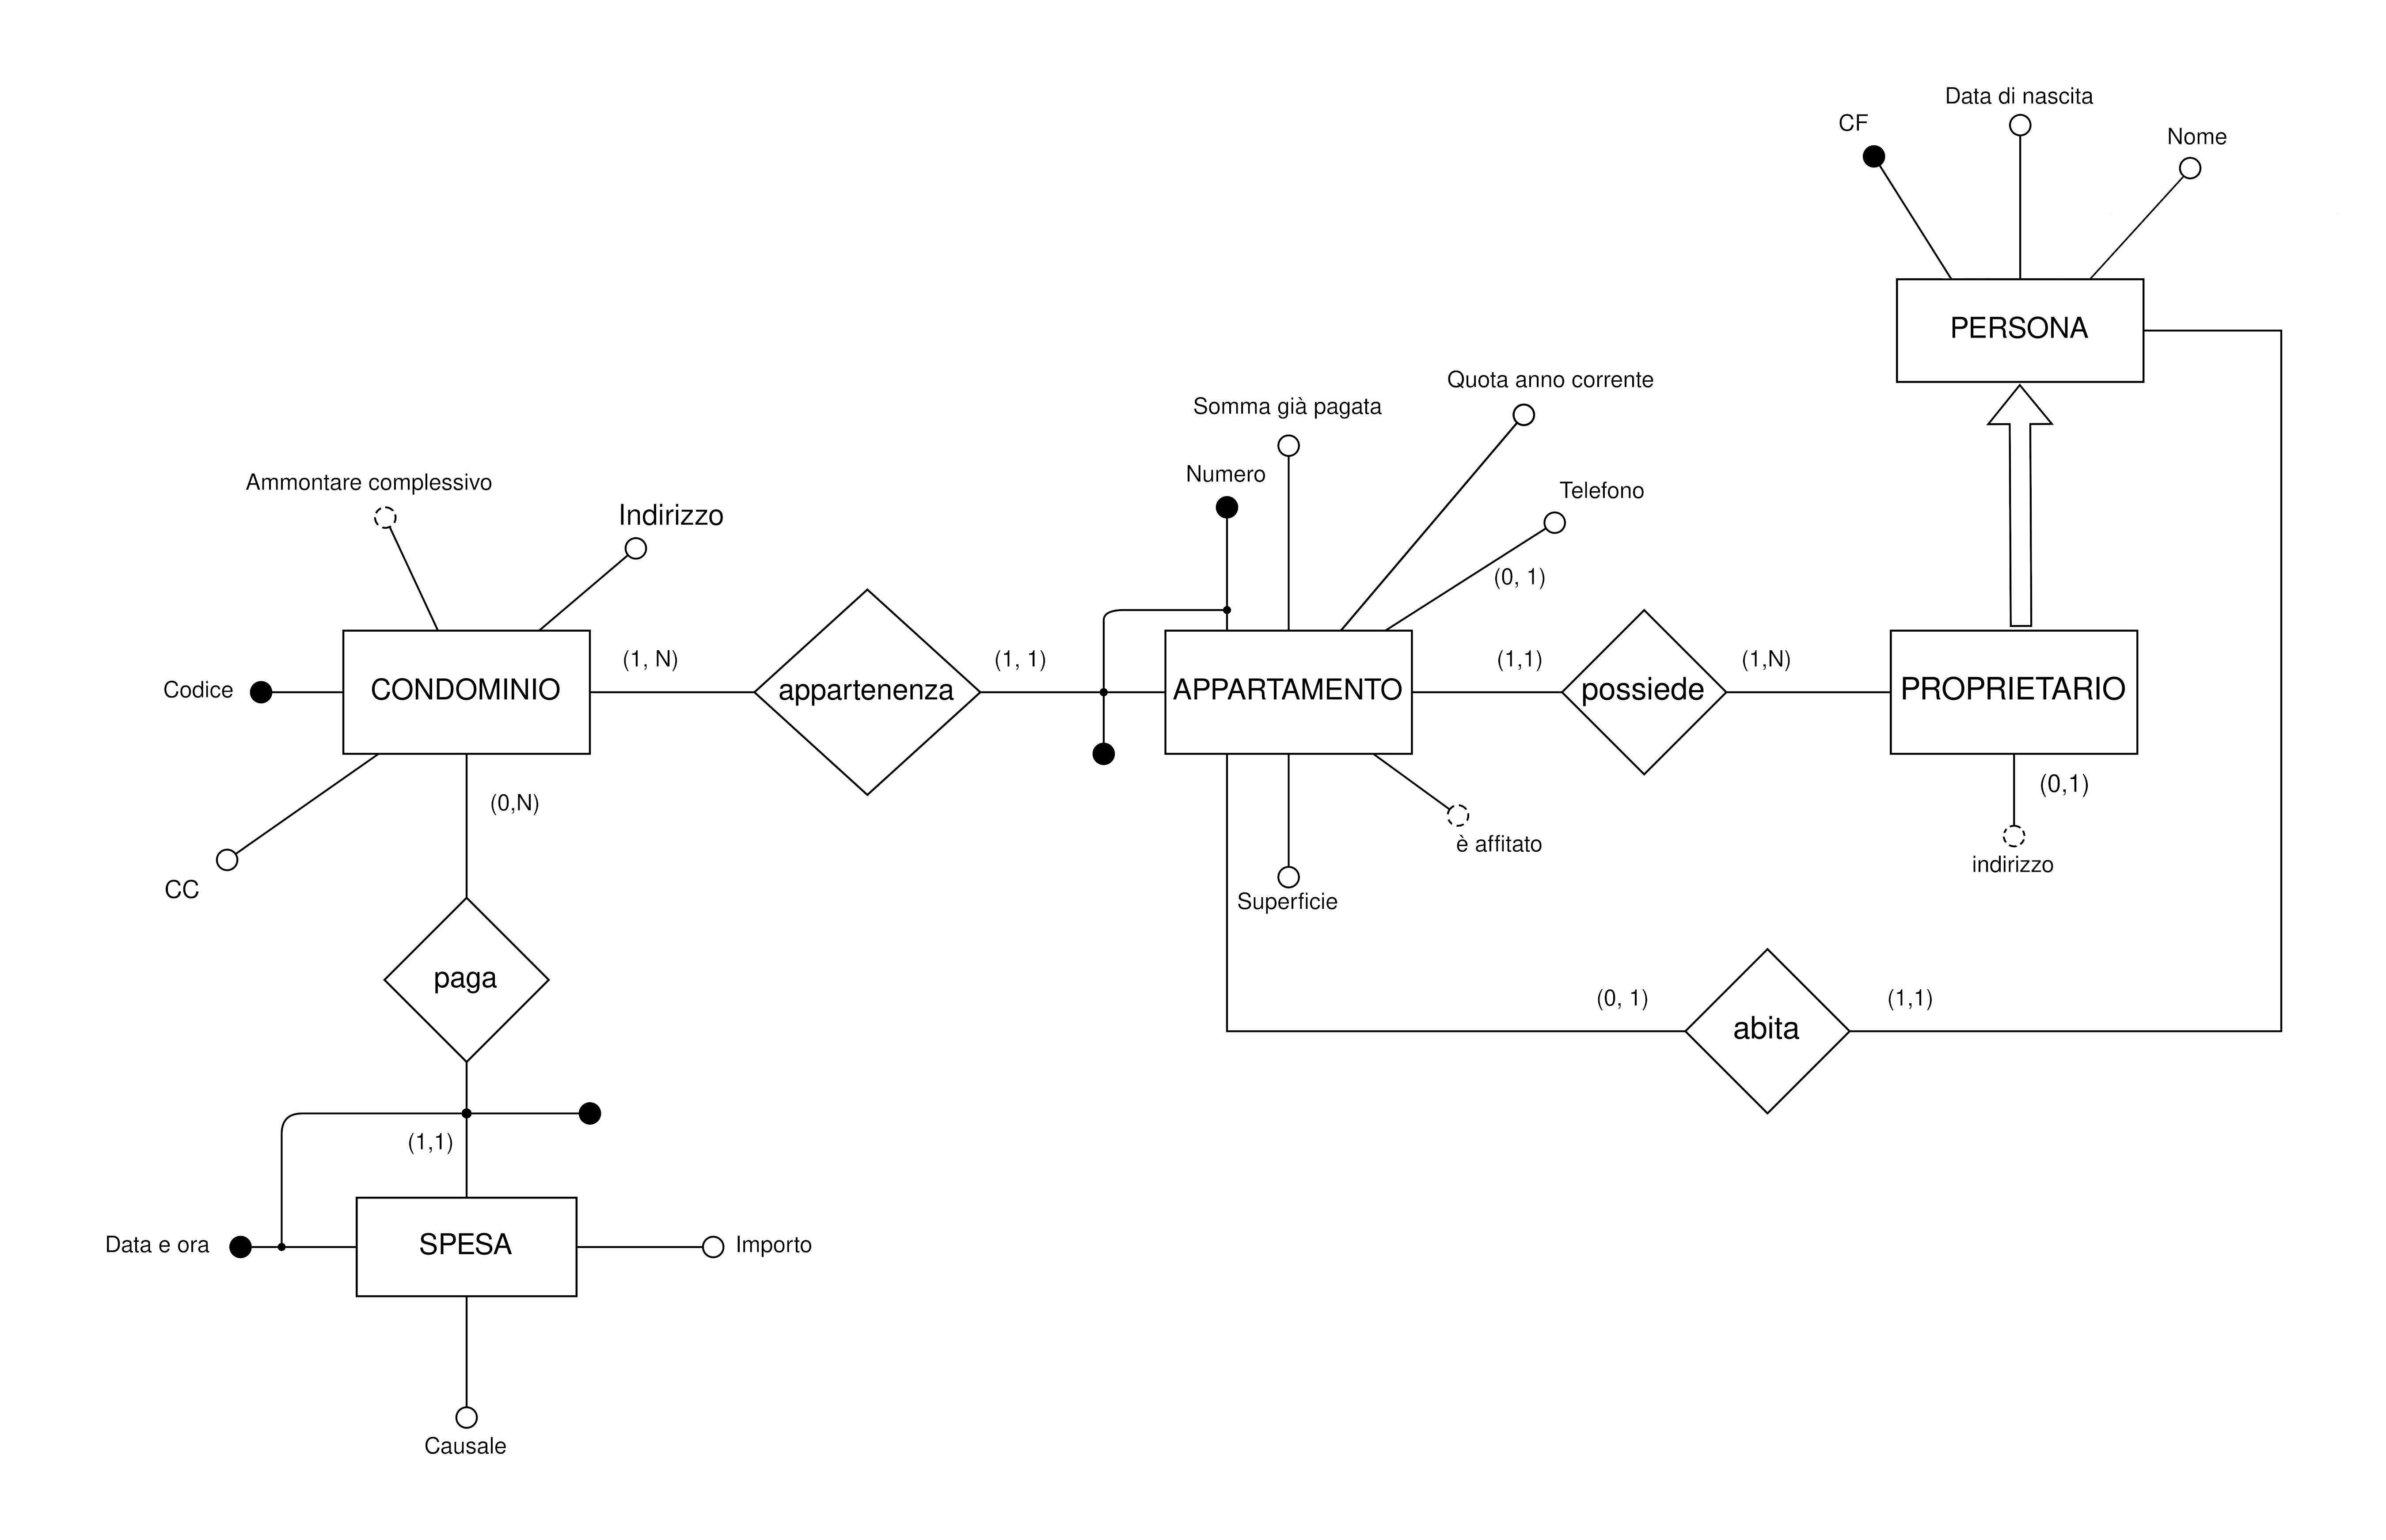
\includegraphics[width=14cm]{ER.png}
	\caption{Schema ER}
\end{figure}

\subsection{Le entità}

\begin{itemize}
    \item Condominio: rappresenta un intero condominio, ed è identificato dal suo codice, e caratterizzato indirizzo, CC, 
                      e l'ammontare complessivo, cioè la somma delle quote già pagate di ogni appartamento di quel condominio.
    \item Spesa: rappresenta la spesa che ogni condominio deve pagare, caratterizzato da importo e causale.
                 È un entità debole di condominio, identificato anche da data e ora.
    \item Appartamento: rappresenta un appartamento di un particolare condominio, è un'entità debole di Condominio, identificato anche da numero.
                        Inoltre, è caratterizzato dall'attributo opzionale telefono, dalla superficie dell'appartamento, 
                        dalla quota dell'anno corrente, la somma che ha già pagato per quell'anno, e da è affittato, un valore booleano
                        che dà vero se nell'appartamento ci abita una persona che non è proprietario di quell'appartamento, e falso altrimenti.
    \item Persona: rappresenta una persona, ed è identificato da CF, e caratterizzato dal suo nome e data di nascita.
    \item Proprietario: è la specializzazione parziale di persona, e quindi mantiene gli attributi di quest'ultimo,
                        con in aggiunta l'attributo indirizzo, derivato e opzionale, che se presente,
                        indica l'indirizzo del condominio a cui appartiene l'appartamento in cui vive.                        
\end{itemize}

\subsection{Le relazioni}

\begin{itemize}
	\item Paga: relazione uno a molti, con partecipazione opzionale dell'entità condominio. Identifica le spese pagate da un determinato condominio. Un condominio può avere più spese pagate, mentre una determinata spesa riguarda un solo condiminio.
 	\item Appartenenza: relazione uno a molti, serve a rappresentare quali appartamenti appartengono a un determinato condominio. A un condominio possono appartenere più appartamenti (e almeno uno per condominio), mentre un appartamento può appartenere solo a un condominio.
  	\item Possiede: relazione uno a molti, identifica quali appartamenti possiede un proprietario. Un proprietario possiede uno o più appartamenti, mentre un singolo appartamento appartiene a un proprietario.
   	\item Abita: relazione uno a uno, con partecipazione opzionale dell'entità appartamento. Un appartamento può essere vuoto, oppure ci può abitare una persona, e una persona può abitare in uno e un solo appartamento.
\end{itemize}


\section{Analisi ridondanze}

\subsection{Tabella operazioni}

% TODO: scegliere codici condominiali

\begin{tabular}{|p{300pt}|l|}
	\hline
	\textbf{Operazione} & \textbf{Frequenza} \\ \hline
	Modifica la quota dell'anno corrente dell'appartamento n° 3 del condominio "X" & 45 volte/mese \\ \hline
	Cancella condominio con codice "Y" & 0.2 volte/anno \\ \hline
	Inserimento Appartamento & 1 volta/anno \\ \hline
	Query ammontare complessivo di tutti i condomini (calcolarlo) & 4 volte/anno \\ \hline
	Query indirizzo di tutti i proprietari & 1 volta/giorno \\ \hline
	Query dato x proprietario per ogni condominio avente almeno 1 app. posseduto da x, elencare le ultime 5 spese dal registro spese & 2 volte/mese \\ \hline
	Query elenco spese dell'anno corrente dei condomini che possiedono almeno 10 appartamenti & 1 volta/anno \\ \hline
	Query importo complessivo delle spese di tutti i condomini con $50 <= ammontareComplessivo <= 100$ & 5 volte/anno \\ \hline
	Query elenco persone che possiedono l'appartamento in cui abitano & 3 volte/anno \\ \hline
	Query elenco persone più anziane che possiedono un appartamento con $superficie >= 50$ & 2 volte/mese \\ \hline
\end{tabular}

\subsection{Tabella valori}

\begin{tabular}{|l|l|l|}
	\hline
	Concetto & Tipo & Volume \\ \hline
	Persona & Entità & 1000 \\ \hline
	Proprietario & Entità & 200 \\ \hline
	Appartamento & Entità & 1500 \\ \hline
	Condominio & Entità & 150 \\ \hline
	Spesa & Entità & 4500 \\ \hline
	abita & Relazione & 1000 \\ \hline
	possiede & Relazione & 1500 \\ \hline
	appartenenza & Relazione & 1500 \\ \hline
	paga & Relazione & 4500 \\ \hline
\end{tabular}

\subsection{Analisi ridondanza sull'attributo derivato Ammontare complessivo di Condominio}

L'analisi delle ridondanze è stata effettuata tenendo in considerazione l'attributo derivato Ammontare-Complessivo dell'entità Condominio, andando a calcolare il costo delle seguenti due operazioni nel caso in cui è presente l'attributo derivato oppure no:

\begin{samepage}
	
\begin{itemize}
	
	\item OP1 := inserimento Appartamento
	\item OP2 := calcolare ammontare complessivo di un Condominio

\end{itemize}

\end{samepage}

Con frequenza rispettivamente di 1 volta/anno e 4 volte/anno

La seguente tabella ci sarà utile in seguito per calcolare il costo delle operazioni.
| Operazione    | Costo (u) |
|---------------|-----------|
| Scrittura (w) | 2         |
| Lettura (r)   | 1         |

L'obbiettivo che ci poniamo è quello di dimostrare che tenere l'attributo derivato sia computazionalmente vantaggioso, nel caso delle due operazioni in esame. Focalizziamo la nostra attenzione sulle entità **Condominio** e **Appartamento** e sulla relazione **Appartenenza**.

***Costo delle due operazione nel caso in cui la ridondanza venga tolta***

Per quanto riguarda l'operazione 1 abbiamo bisogno di un accesso in scrittura all'entità Appartamento e un accesso in scrittura alla relazione Appartenenza.

Per quanto riguarda l'operazione 2 serve un accesso in lettura all'entità Condominio, per ricavare il condominio in questione e 10 letture alla relazione Appartenenza (ottenuto dividendo il volume dell'entità Appartamento per il volume dell'entità Condominio).

Quindi,

\begin{verbatim}
	
> Costo_OP1 = 2w
> 
> Costo_OP2 = 1r + (1500/150)r = 11r

\end{verbatim}

Andando a moltiplicare i costi per le relative frequenze delle due operazioni e tenendo in considerazione la tabella subito sopra

\begin{verbatim}
	
> Costo_OP1 = 2 * 2 * 1 volta/anno = 4 accessi all'anno
> 
> Costo_OP2 = 11 * 1 * 4 volte/anno = 44 accessi all'anno
>
> Costo_TOT_senza_rid = 48 accessi all'anno

\end{verbatim}

***Costo delle due operazione nel caso in cui la ridondanza venga mantenuta***

Per quanto riguarda l'operazione 1 abbiamo bisogno di un accesso in scrittura all'entità Appartamento (per inserire l'appartamento), un accesso in scrittura alla relazione Appartenenza (per memorizzare la coppia condominio-appartamento), un accesso in lettura all'entità Condominio (per cercare il condominio in questione) e un accesso in scrittura all'entità Condominio (sommando all'attributo derivato il valore dell'attributo Quota-anno-corrente dell'appartamento appena inserito).

Per quanto riguarda l'operazione 2 serve un solo accesso in lettura all'entità Condominio, per leggere il contenuto dell'attributo derivato Ammontare-complessivo.

Quindi,

\begin{verbatim}

> Costo_OP1 = 1r + 3w
> 
> Costo_OP2 = 1r

\end{verbatim}

Andando a moltiplicare i costi per le relative frequenze delle due operazioni e tenendo in considerazione la tabella subito sopra

\begin{verbatim}
	
> Costo_OP1 = 1 + (3 * 2) * 1 volta/anno = 7 accessi all'anno
> 
> Costo_OP2 = 1 * 4 volte/anno = 4 accessi all'anno
>
> Costo_TOT_con_rid = 11 accessi all'anno

\end{verbatim}

E quindi siccome $Costo\_TOT\_con\_rid < Costo\_TOT\_senza\_rid$ allora conviene mantenere l'attributo derivato Ammontare-complessivo.

\section{Schema logico relazionale}

Lo schema logico permette di rappresentare i concetti derivanti dallo schema ER
nel modello logico utilizzato dalla base di dati.

In questo progetto viene utilizzato il modello relazionale il quale utilizza le relazioni
(o tabelle) e le associazioni fra di esse per rappresentare i dati richiesti dal modello
concettuale.

Il seguente schema logico ha tradotto le entità dello schema ER in tabelle, e le relazioni
di tipo 1 a N dall'entità A all'entità B in associazioni tra la chiave esterna di A che
fa riferimento alla chiave primaria di B.

In questo schema ER è presente una singola specializzazione parziale di Persona in
Proprietario pertanto viene unita al genitore, e tutti gli attributi e relazioni del figlio
ora sono sono del genitore.

L'attributo condominio.ammontareComplessivo è un attributo derivato ma è comunque presente
nello schema logico in quanto lo studio sulla ridondanza ha sottolineato che mantenerlo porta
una maggiore efficienza computazionale della basi di dati.

\begin{itemize}

\item condominio(\underline{codice}, contoCorrente, indirizzo, ammontareComplessivo)

\item spesa(\underline{dataOra, \textit{condominio}}, importo, causale)

\item appartamento(\underline{numero, \textit{condominio}}, quotaAnnoCorrente, sommaPagata, telefono, superficie, \textit{proprietario})

\item persona(\underline{cf}, nome, dataNascita, indirizzo, \textit{numeroAppartamento, condominio})

\end{itemize}

\subsection{Chiavi esterne}

Di seguito sono elencate le chiavi esterne, la freccia indica che l'attributo (o l'insieme di attributi)
a sinistra è chiave esterna dell'entità a destra

% TODO: usare o no le parentesi graffe

\begin{itemize}
	\item spesa.condominio $\implies$ condominio
	\item appartamento.condominio $\implies$ condominio
	\item appartamento.proprietario $\implies$ persona
	\item $\{$persona.numeroAppartamento, persona.condominio$\}$ $\implies$ appartamento
\end{itemize}



\section{Progettazione fisica}

\section{Implementazione in SQL}

\section{Analisi dati}

\end{document}